\documentclass[master.tex]{subfiles}
\begin{document}

\chapter{Example Formal System --- Propositional Logic}
\label{chap:example_propositional_logic}

Once you are familiar with some basic features and usability of \emph{Phometa}
from the last chapter. This chapter aims to show more advance features on
another formal system named \emph{Propositional Logic} which is the most well
known logical system\footnote{Logical system is a formal system together with
  semantics\supercite{formal-system-wiki}}.

Logic, in general, works so well with traditional derivation system, hence there
is spacial name called \emph{Natural Deduction} which is a combination of any
kind of Logic together with derivation system.

\section{Grammars}

As usual, the first thing that needed to be defined is syntax which consists of
several grammars. Propositional logic has \pgmr{Prop}, \pgmr{Atom},
\pgmr{Context}, and \pgmr{Judgement} as its grammars.

\pgmr{Prop} is a proposition, semantically, it is a term that can be evaluated
to either true or false (given that there are no variables in the term).
Grammars of \pgmr{Prop} can be defined in Phometa as the following

\centerline{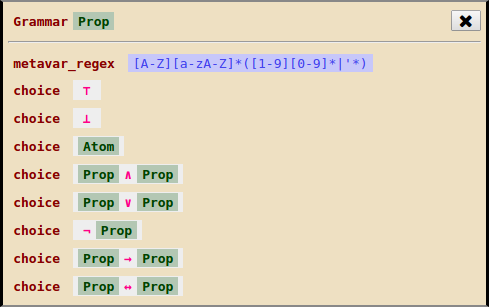
\includegraphics[scale=0.5]{prop-grammar-prop.png}}

This grammar is equivalence to the following Backus Normal Form
\begin{lstlisting}[style=bnf]
<Prop> ::= $\top$ | $\bot$ | <Atom>
         | <Prop> $\wedge$ <Prop>
         | <Prop> $\vee$ <Prop>
         | $\neg$ <Prop>
         | <Prop> $\rightarrow$ <Prop>
         | <Prop> $\leftrightarrow$ <Prop>
         | meta-variables comply with regex
             /[A-Z][a-zA-Z]*([1-9][0-9]*|'*)/
\end{lstlisting}

\newcommand{\propTop}[0]{\bat{\pifmt{$\top$}}}
\newcommand{\propBot}[0]{\bat{\pifmt{$\bot$}}}
\newcommand{\propAnd}[0]{\pifmt{$\wedge$}}
\newcommand{\propOr}[0]{\pifmt{$\vee$}}
\newcommand{\propNot}[0]{\pifmt{$\neg$}}
\newcommand{\propImp}[0]{\pifmt{$\rightarrow$}}
\newcommand{\propIff}[0]{\pifmt{$\leftrightarrow$}}

We take advantage of visualisation by replacing brackets with underlines, this
should improve readability because reader can see a whole term in a compact
way but still able check how they are bounded when needed, for example,
\begin{itemize}
  \item \propTop{} represents $(\top)$
  \item \propBot{} represents $(\bot)$
  \item \bat{\propTop\propAnd\propBot} represents $((\top) \wedge (\bot))$
  \item \bat{\propBot\propOr\bat{\propTop\propOr\propBot}}
    represents $((\bot) \vee ((\top) \vee (\bot)))$
  \item \bat{\bat{\propTop\propAnd\propTop}\propImp\propBot}
    represents $(((\top) \wedge (\top)) \rightarrow (\bot))$
  \item and so on \dots
\end{itemize}

Having only close terms is not so useful, so we allow terms to have
meta-variables, when this is the case, we can see these terms as \emph{pattern},
for example,
\begin{itemize}
  \item \pvar{A} represents arbitrary \pgmr{Prop} term
  \item \bat{\propNot\pvar{A}} represents \pgmr{Prop} term that has
    \propNot\ as main connector
  \item \bat{\pvar{A}\propAnd\pvar{B}} represents \pgmr{Prop} term that has
    \propAnd\ as main connector
  \item \bat{\pvar{A}\propAnd\pvar{A}} represents \pgmr{Prop} term that has
    \propAnd\ as main connector and both of its sub-terms are identical
  \item and so on \dots
\end{itemize}

Meta-variables names must comply to regular expression stated in \kVarRegex\ of
corresponding grammar declaration, this allow us to enforce some naming
convention, for example, meta-variables of \pgmr{Prop} must start with capital
letter.

Next, we would like to create the grammar for \pgmr{Atom}. Intuitively, an atom
is primitive truth statement that can be either true or false. we can define
\pgmr{Atom} like the following.

\centerline{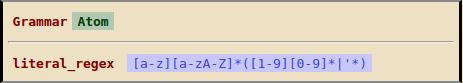
\includegraphics[scale=0.5]{prop-grammar-atom.png}}

\pgmr{Atom} definition doesn't neither \kMetaVarRegex{} or \kChoice{}s

we can represent
it as a grammar that doesn't have any choice, hence, using meta-variable become
the only way to instantiate \pgmr{Atom}. (TODO:\ replace this with the real
screenshot)

At this stage, reader might wonder that what is different between meta-variable
of \pgmr{Prop} and \pgmr{Atom} choice in \pgmr{Prop}, well, meta-variable is
something that can be substituted later while \pgmr{Atom} it truth statement that
is static. For example,
if we know that \bat{\pvar{A}\propOr\bat{\propNot\pvar{A}}} holds, we can derive
corresponding term such as \bat{\propTop\propOr\bat{\propNot\propTop}},
\bat{\bat{\pvar{raining}}\propOr\bat{\propNot\bat{\pvar{raining}}}},
\bat{\bat{\pvar{B}\propAnd\pvar{C}}\propOr\bat{\propNot\bat{\pvar{B}\propAnd\pvar{C}}}}
directly, but knowing
\bat{\bat{\pvar{raining}}\propOr\bat{\propNot\bat{\pvar{raining}}}} doesn't
help us to derive something like the former case does. In order to prevent this
confusion we set \kVarRegex\ of \pgmr{Prop} and \pgmr{Atom} differently, so if
user accidentally write \pvar{p} on a hole that require \pgmr{Prop}, Phometa
will raise an error messages and user can fix it.

(TODO:\ ask Dr Krysia, the reason above doesn't prevent meta-variable of atom to
be substituted by another meta-variable of atom, this problem also rise when I
try to combine \prule{hypothesis-base} and hypothesis next together. I am
thinking to create another kind of meta-variable that doesn't allow substitution
(maybe under name \pkw{name\_regex}) such that meta-variable under this regular
expression cannot be substituted)

Now, we have enough ingredient to create a proper proposition, one might say
that we can start proving it directly, however, most of proposition that we will
dealing with only holds under certain assumptions, hence, a \emph{judgement}
should be in the form $A_1, A_2, ..., A_n \vdash B$ where $A_{1..n}$ are
assumptions and $B$ is conclusion.

To model a judgement in Phometa, first we need to model assumptions or in the
other name, \pgmr{Context} as the following (TODO:\ replace this with the real
screenshot)

\centerline{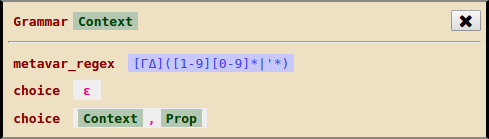
\includegraphics[scale=0.5]{prop-grammar-context.png}}

\newcommand{\propEmptyContext}{\bat{\pifmt{$\epsilon$}}}

So a term of \pgmr{Context} can be either empty context or another context
appended by a proposition. We can see a context as a list of proposition.

Now we are ready to define \pgmr{Judgement} as the following (TODO:\ replace
this with the real screenshot)

\centerline{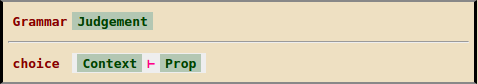
\includegraphics[scale=0.5]{prop-grammar-judgement.png}}

\newcommand{\propTurnstile}{\pifmt{$\vdash$}}

Examples of \pgmr{Judgement} term could be like
\begin{itemize}
  \item \bat{\bat{\bat{\propEmptyContext\pifmt{,}\bat{\pvar{p}}}\pifmt{,}\bat{\bat{\pvar{p}}\propImp\bat{\pvar{q}}}}\propTurnstile\bat{\pvar{q}}}

  assume atom \pvar{p} and proposition \bat{\bat{\pvar{p}}\propImp\bat{\pvar{q}}} then atom \pvar{q} holds

  \item \bat{\bat{\propEmptyContext\pifmt{,}\bat{\pvar{B}\propAnd\pvar{A}}}\propTurnstile\bat{\pvar{A}\propAnd\pvar{B}}}

  let \pvar{A} and \pvar{B} be arbitrary \pgmr{Prop} and assume that
      \bat{\pvar{B}\propAnd\pvar{A}} then \bat{\pvar{A}\propAnd\pvar{B}}
      holds

  \item \bat{\propEmptyContext\propTurnstile\bat{\pvar{A}\propOr\bat{\propNot\pvar{A}}}}

  let \pvar{A} be arbitrary \pgmr{Prop} then
  \bat{\pvar{A}\propOr\bat{\propNot\pvar{A}}} holds

\end{itemize}

Please note that \pgmr{Judgement} doesn't have field \kVarRegex so we can't
accidentally use meta-variable for \pgmr{Judgement}.

\section{Input method of a term}

When a term is created, it can be in one of this mode

\subsection{Editable up to Grammars}
On this mode, we have a absolute control over a term i.e.\ both of grammar and
term content can be changed, when it is created it will look like this,

\centerline{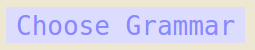
\includegraphics[scale=0.25]{term-input-method-001.png}}

This is a completely blank term, we can set its grammar by clicking on it, then
you will see option on keymap-pane (left-bottom corner of screen) as the following

\centerline{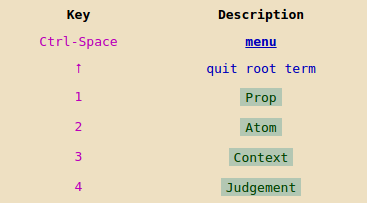
\includegraphics[scale=0.5]{term-input-method-002.png}}

This show all of possible key-blinding including all of grammar that can be use,
now we will select \pgmr{Prop} for this term's grammar by press \emph{1}
(or alternatively clicking on \pgmr{Prop} directly), which now tern the
term to be like this

\centerline{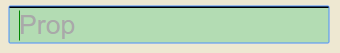
\includegraphics[scale=0.25]{term-input-method-003.png}}

This means the term now know that it is \pgmr{Prop} term and hasn't know a
content, and in order give a content we can set it to be either a construction
term or meta-variable term. Now let make it a construction term, if you see
keymap-pane again, it will look like this

\centerline{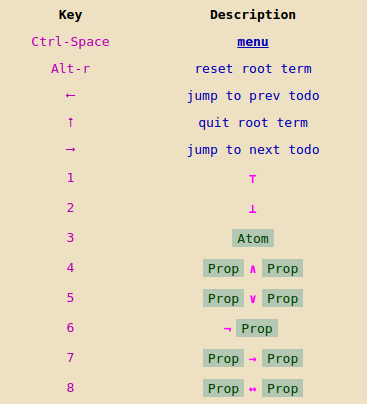
\includegraphics[scale=0.5]{term-input-method-004.png}}

Similar to grammar selection, we can press the corresponded key-blinding that
construct the term as we like. Let press \emph{7} for \bat{\pgmr{Prop}
  \pifmt{$\rightarrow$} \pgmr{Prop}} and now the term become like this,

\centerline{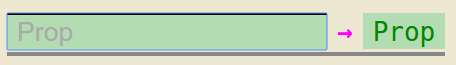
\includegraphics[scale=0.25]{term-input-method-005.png}}

The root term now has \pifmt{$\rightarrow$} as the main connector and
\emph{todos} spilt into two place, this process is recursive, you can try to
split it again by e.g. press \emph{5} for \bat{\pgmr{Prop}
  \pifmt{$\wedge$} \pgmr{Prop}} and get

\centerline{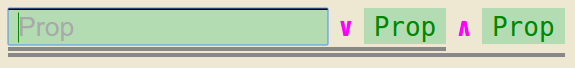
\includegraphics[scale=0.25]{term-input-method-006.png}}

We also be able to move to other todos by clicking on target todo or simply
press left arrow or right arrow for previous and next todo respectively.

Next, we can make it to be meta-variable term by enter meta-variable name on the
target todo then press enter. Let type \emph{A} for the first todo

\centerline{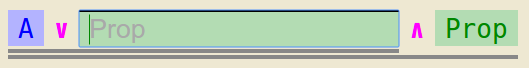
\includegraphics[scale=0.25]{term-input-method-007.png}}

Now the first term become meta-variable and the cursor move to the next one
automatically, please note that the meta-variable name must comply to \kVarRegex
of corresponding grammar, otherwise, it will not convert to meta-variable. If
you want to create an atom here, you can't just type directly since it is for
\pgmr{Prop} meta-variable (As you can see from background text in todo),
instead, you need to press \emph{3} to tell Phometa that it is construction for
\pgmr{Atom}, like this

\centerline{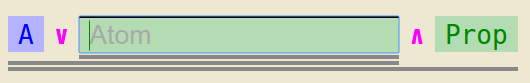
\includegraphics[scale=0.25]{term-input-method-008.png}}

Now the background of current todo change from \emph{Prop} to \emph{Atom} and
has extra underline so now you can type and atom

\centerline{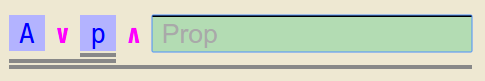
\includegraphics[scale=0.25]{term-input-method-009.png}}

Not only meta-variable that can finish up todos, some of grammar choice just
doesn't have sub-term, we could finish the last todo, by just press \emph{1} for \propTop

\centerline{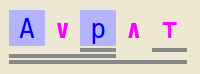
\includegraphics[scale=0.25]{term-input-method-010.png}}

Now the term is finished, you can still return to the term and click some of
them e.g.\ clicking \pvar{A}

\centerline{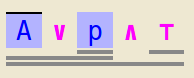
\includegraphics[scale=0.25]{term-input-method-011.png}}

You can navigate to parent term my press up-arrow

\centerline{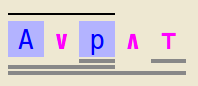
\includegraphics[scale=0.25]{term-input-method-012.png}}

If you think you create some sub-term wrongly, you click on the that sub-term
(in this is case \bat{\pvar{A} \propOr \bat{\pvar{p}}}) then press \emph{Alt-t}

\centerline{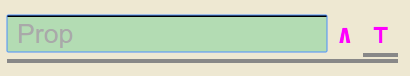
\includegraphics[scale=0.25]{term-input-method-013.png}}

Or if everything is wrong including the root term grammar, you just press
\emph{Alt-r}, this will go back to \emph{asking for grammar state}

\centerline{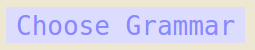
\includegraphics[scale=0.25]{term-input-method-001.png}}

To give more example, let try to create \pgmr{Judgement} term, by click \emph{4}

\centerline{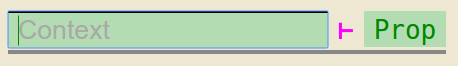
\includegraphics[scale=0.25]{term-input-method-014.png}}

You might expect that after pressing \emph{4}, it should be just green area with
background written as \emph{Judgement}, why it is auto expend like this, well,
we have spacial case that if selecting grammar as just one choice and can't be
meta-variable (we didn't state \kVarRegex\ for \pgmr{Judgement}), it will auto
expend to that choice since that is the only action available.

\subsection{Editable up to Term}
This mode is the the same as editable up to grammar except that the grammar is
given and we can't change it. If we try to reset the whole term \emph{Alt-r}, it
the grammar still remain there.

\subsection{Read only}
In this mode, you can just view the term and nothing else.

\section{The first theorem}

Grammars provide rigorous way to construct well-formed terms, however these
terms doesn't have any meaning, the way to give the its meaning to prove that it
is \emph{valid}. Validity of each term depends on its grammars, for example,
a \pgmr{Prop} term is valid iff that term always evaluate to true, a
\pgmr{Judgement} term is valid iff assuming all propositions form left hand
side then the proposition on the right hand side hold.

The main idea of proving in Phometa is that you state (in a theorem) that some
term is valid, then give a reason why it is valid, this can be done by either
\emph{Prove by Rule} or \emph{Prove by Lemma}.

A rule is a meta-statement which say that, if some terms (premises) is valid
then the conclusion term is valid.

We want ability to state that for any proposition that is in assumptions, it can
be conclusion i.e. $A_{1..n} \vdash A_i$ where $i \in {1..n}$

This is achievable by \prule{hypothesis-base} and \prule{hypothesis-next}

\node{
  \kRule \pstr{hypothesis-base}
}{
  \kConclude & \bat{
        \bat{\pvar{$\Gamma$} \pifmt{,} \pvar{A}}
        \pifmt{$\vdash$}
        \pvar{A}
    } \\
}

This state that if we have a \pgmr{Judgement} such that the last proposition in
context is identical to the conclusion proposition, then that \pgmr{Judgement}
is valid.

\node{
  \kRule \pstr{hypothesis-next}
}{
  \kPremise & \bat{
        \pvar{$\Gamma$}
        \pifmt{$\vdash$}
        \pvar{A}
    } \\

  \kConclude & \bat{
        \bat{\pvar{$\Gamma$} \pifmt{,} \pvar{B}}
        \pifmt{$\vdash$}
        \pvar{A}
    } \\
}

This state that if we have a valid \pgmr{Judgement}, then appending the another
proposition in the context still valid

So let prove the very first judgement
\bat{\bat{\propEmptyContext\pifmt{,}\pvar{A}}\propTurnstile\pvar{A}}


TODO:\ continue here

At this stage, you might think that validity is necessary only for the
grammars that have a truth value, e.g.\ it doesn't make sense to prove a
\pgmr{Context} term. Well, this is because we know that every well-form
\pgmr{Context} term is valid term. Generally, this is not always be the
case, for example, if we define an algebra of integer like this

\node{
    \kGrammar \pstr{Int}
} {
    \kVarRegex & \pregex{a-z} \\

    \kChoice & \bat{\pifmt{0}} \\

    \kChoice & \bat{\pifmt{1}} \\

    \kChoice & \bat{\pgmr{Int} \pifmt{+} \pgmr{Int}} \\

    \kChoice & \bat{\pgmr{Int} \pifmt{-} \pgmr{Int}} \\

    \kChoice & \bat{\pgmr{Int} \pifmt{$\times$} \pgmr{Int}} \\

    \kChoice & \bat{\pgmr{Int} \pifmt{$\div$} \pgmr{Int}} \\
}

Obviously, \pgmr{Int} doesn't have truth value, nevertheless, not every
\pgmr{Int} term is valid e.g. \bat{\pvar{n} \pifmt{$\div$} \bat{\pifmt{0}}}, so
we need to provide rules to \emph{verify} \pgmr{Int}.

\end{document}